\documentclass[a4paper,11pt]{article}

\usepackage[margin=2.4cm]{geometry}
\usepackage{graphicx}
\usepackage{booktabs}
\usepackage{array}
\usepackage{xcolor}
\usepackage{amsmath}
\usepackage{hyperref}
\usepackage{caption}
\usepackage{subcaption}
\usepackage{float}

\hypersetup{colorlinks=true, linkcolor=blue, citecolor=blue, urlcolor=blue}
\setlength{\parskip}{0.5em}
\setlength{\parindent}{0em}

\newcommand{\modelbase}{TranAD}
\newcommand{\modele}{TranAD-Ensemble}
\newcommand{\modelcode}{TranAD\_E}
\newcommand{\pos}[1]{\textcolor{green!45!black}{#1}}
\newcommand{\neg}[1]{\textcolor{red!70!black}{#1}}

\title{\textbf{Stage Report on Critical Transition Forecasting in Complex Systems}\\
\large Preliminary Results of TranAD-Ensemble with Top-k Anomaly Score Aggregation}
\author{Stage Research Report}
\date{\today}

\begin{document}
\maketitle

\begin{abstract}
This report summarizes the current progress of a research direction focused on
\textit{using artificial intelligence methods and the theory of critical events for critical transitions forecasting in complex systems}. The current stage uses TranAD as the baseline model for multivariate time-series anomaly detection and evaluates a lightweight variant, TranAD-Ensemble, combined with top-k anomaly score aggregation. In the implementation and experiment logs, this model is denoted as \texttt{TranAD\_E}, where \texttt{E} stands for \textit{Ensemble}.

The purpose of this stage is not to replace the TranAD architecture with a substantially different model. Instead, the goal is to test whether a small modification to the output stage, together with a more localized anomaly score aggregation rule, can improve the detection of potential critical-event signals in complex systems.

Experiments were conducted on SMD, MSL, Synthetic, SWaT, NAB, and MBA datasets. TranAD-Ensemble with top-k aggregation slightly improves F1 score on Synthetic and MBA, remains unchanged on MSL, SWaT, and NAB, and decreases performance on SMD. These results indicate that the current modification is partially effective but not yet robust across all datasets.
\end{abstract}

\section{Research Context}

Critical transitions in complex systems refer to abrupt changes in system state, often caused by the accumulation of weak but meaningful early-warning signals. Examples include industrial control failures, spacecraft telemetry anomalies, server faults, and other high-dimensional system instabilities.

From a machine learning perspective, critical transition forecasting can be approached as an early anomaly detection problem in multivariate time series. The model should identify abnormal temporal patterns before they evolve into severe system-level transitions. In this setting, anomalous observations can be treated as empirical proxies of critical events.

TranAD is selected as the baseline model because it provides a compact and interpretable reconstruction-based framework for multivariate anomaly detection. Its two-phase self-conditioning mechanism allows the model to reconstruct the current time window while using reconstruction discrepancy as additional context.

\section{Baseline Model: TranAD}

TranAD receives a sliding input window $X \in \mathbb{R}^{W \times F}$, where $W$ is the window length and $F$ is the number of variables. The model first produces a phase-1 reconstruction $\hat{X}^{(1)}$. Then it computes a self-conditioning signal:

\begin{equation}
    C = (\hat{X}^{(1)} - X)^2.
\end{equation}

This signal is used in the second decoding phase to produce the final reconstruction $\hat{X}^{(2)}$. The baseline anomaly score is computed from the reconstruction error:

\begin{equation}
    E_{t,f} = (X_{t,f} - \hat{X}^{(2)}_{t,f})^2.
\end{equation}

The baseline structure is shown in Figure~\ref{fig:arch_base}.

\begin{figure}[H]
    \centering
    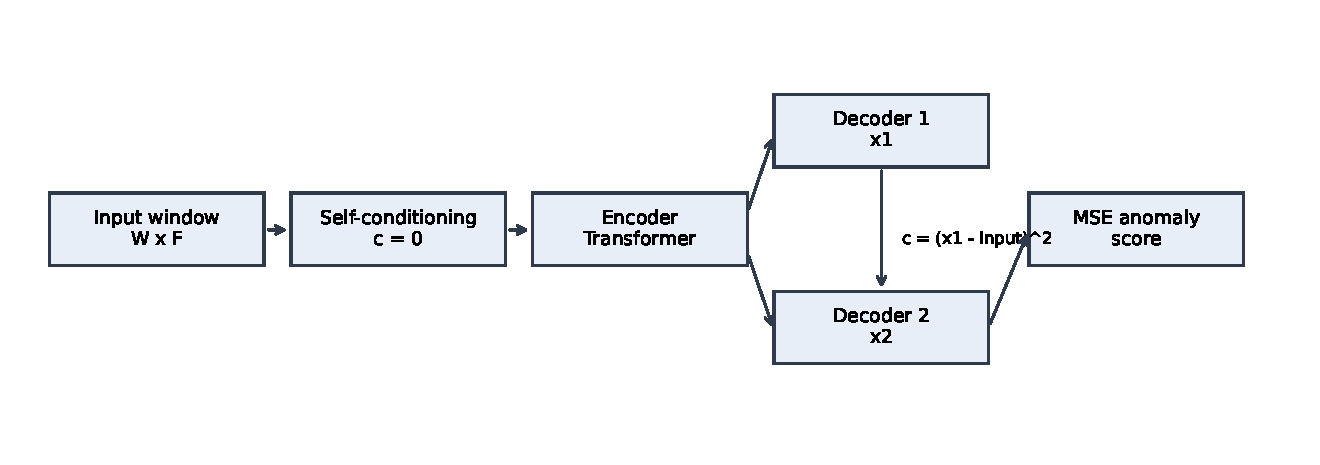
\includegraphics[width=0.95\linewidth]{figures/architecture_tranad.pdf}
    \caption{Baseline TranAD architecture.}
    \label{fig:arch_base}
\end{figure}

\section{Proposed Stage Variant: TranAD-Ensemble with Top-k Aggregation}

The current stage evaluates one focused variant: TranAD-Ensemble with top-k anomaly score aggregation. In the codebase this variant is named \texttt{TranAD\_E}. The letter \texttt{E} means \textit{Ensemble}, because the modification introduces a learnable ensemble of the two TranAD reconstruction phases. Other experimental variants are intentionally excluded from this report.

\subsection{Phase-Output Ensemble}

TranAD-Ensemble keeps the original two-phase TranAD structure but introduces a learnable output ensemble between phase-1 and phase-2 reconstructions:

\begin{equation}
    \hat{X} = (1-\alpha)\hat{X}^{(1)} + \alpha \hat{X}^{(2)}, \quad
    \alpha = \sigma(\theta),
\end{equation}

where $\theta$ is a learnable scalar and $\sigma(\cdot)$ is the sigmoid function. The motivation is that phase-1 and phase-2 outputs may capture different reconstruction behavior. Phase 1 is closer to direct reconstruction, while phase 2 is conditioned on discrepancy information. A learnable ensemble allows the model to balance both outputs.

\subsection{Top-k Anomaly Score Aggregation}

For multivariate systems, a critical event may be reflected by a small number of key variables rather than by all variables simultaneously. A simple mean over all feature-wise errors may dilute such localized signals. Therefore, the current stage uses top-k aggregation:

\begin{equation}
    S_t^{topk} = \frac{1}{k}\sum_{f \in \operatorname{TopK}(E_{t,1},\ldots,E_{t,F})} E_{t,f}.
\end{equation}

This aggregation computes the final anomaly score using the largest $k$ feature-wise reconstruction errors at each timestamp. In practical terms, top-k aggregation emphasizes the most abnormal variables at each time point.

The modified structure is shown in Figure~\ref{fig:arch_e}.

\begin{figure}[H]
    \centering
    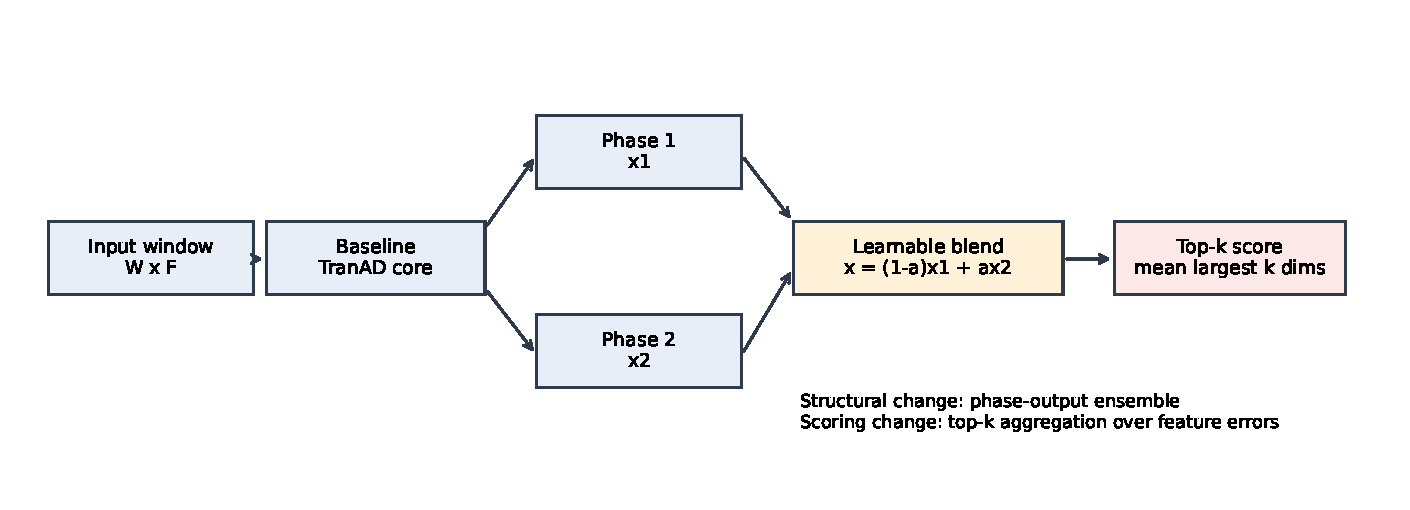
\includegraphics[width=0.98\linewidth]{figures/architecture_tranad_e_topk.pdf}
    \caption{TranAD\_E with top-k anomaly score aggregation.}
    \label{fig:arch_e}
\end{figure}

\section{Datasets}

The experiments use six benchmark datasets that represent different types of complex systems and anomaly patterns.

\textbf{SMD (Server Machine Dataset).}
SMD is a multivariate server monitoring dataset collected from machines in a large-scale Internet service environment. It contains multiple telemetry channels that describe server behavior. Anomalies often correspond to operational faults or abnormal machine states. This dataset is important for evaluating whether a method can detect system-level failures in high-dimensional infrastructure data.

\textbf{MSL (Mars Science Laboratory).}
MSL is a spacecraft telemetry dataset from NASA. It contains multivariate sensor and actuator signals from the Mars Science Laboratory mission. Anomalies in this dataset are related to abnormal spacecraft subsystem behavior. It is relevant to critical transition forecasting because telemetry anomalies may indicate early signs of instability in engineered systems.

\textbf{Synthetic.}
The Synthetic dataset is generated with controlled anomaly injection. It is useful for validating whether a method can detect known abnormal patterns under a cleaner experimental setting. Because the anomaly mechanism is more controlled than in real-world datasets, Synthetic results help separate model behavior from data noise.

\textbf{SWaT (Secure Water Treatment).}
SWaT is an industrial control system dataset collected from a water treatment testbed. It contains sensor and actuator measurements under normal operation and attack scenarios. It is especially relevant to complex-system transition forecasting because attacks or process faults may lead to abrupt changes in system dynamics.

\textbf{NAB (Numenta Anomaly Benchmark).}
NAB contains time-series data from multiple real-world domains, including server metrics, application behavior, and other streaming signals. In this project, NAB is used as a benchmark for evaluating anomaly detection on comparatively smaller or more diverse time-series settings.

\textbf{MBA.}
MBA is a multivariate benchmark dataset used in this project for anomaly detection evaluation. It provides another system setting for testing whether the proposed scoring strategy generalizes beyond the NASA, server, synthetic, and industrial-control datasets.

\section{Experimental Setup}

This report compares only two methods:

\begin{itemize}
    \item \textbf{TranAD}: the baseline model.
    \item \textbf{TranAD-Ensemble + top-k}: TranAD with learnable phase-output ensemble and top-k anomaly score aggregation. The implementation name is \texttt{TranAD\_E}.
\end{itemize}

The evaluation uses Precision, Recall, and F1 score. Experiments were conducted on six datasets: SMD, MSL, Synthetic, SWaT, NAB, and MBA.

The goal of this stage is to identify whether the proposed modification provides useful evidence for further development. The results should therefore be interpreted as preliminary evidence rather than final model validation.

\section{Results}

\subsection{Metric Table}

Table~\ref{tab:metrics} reports the measured performance of TranAD and TranAD-Ensemble with top-k aggregation. TranAD-Ensemble improves slightly on Synthetic and MBA, remains unchanged on MSL, SWaT, and NAB, and decreases on SMD.

\begin{table}[H]
\centering
\caption{Performance comparison between TranAD and TranAD-Ensemble with top-k aggregation.}
\label{tab:metrics}
\small
\begin{tabular}{lccccccc}
\toprule
\textbf{Dataset} &
\textbf{Model} &
\textbf{F1} &
\textbf{Precision} &
\textbf{Recall} &
\textbf{$\Delta$F1} &
\textbf{$\Delta$P} &
\textbf{$\Delta$R} \\
\midrule
SMD & TranAD & 0.9981 & 0.9989 & 0.9974 & -- & -- & -- \\
SMD & TranAD-Ensemble+top-k & 0.9134 & 0.9951 & 0.8440 & \neg{-0.0848} & \neg{-0.0037} & \neg{-0.1534} \\
\midrule
MSL & TranAD & 0.9495 & 0.9038 & 1.0000 & -- & -- & -- \\
MSL & TranAD-Ensemble+top-k & 0.9495 & 0.9038 & 1.0000 & 0.0000 & 0.0000 & 0.0000 \\
\midrule
Synthetic & TranAD & 0.9756 & 0.9524 & 1.0000 & -- & -- & -- \\
Synthetic & TranAD-Ensemble+top-k & 0.9836 & 0.9677 & 1.0000 & \pos{+0.0080} & \pos{+0.0154} & 0.0000 \\
\midrule
SWaT & TranAD & 0.8151 & 1.0000 & 0.6879 & -- & -- & -- \\
SWaT & TranAD-Ensemble+top-k & 0.8151 & 1.0000 & 0.6879 & 0.0000 & 0.0000 & 0.0000 \\
\midrule
NAB & TranAD & 0.9412 & 0.8889 & 1.0000 & -- & -- & -- \\
NAB & TranAD-Ensemble+top-k & 0.9412 & 0.8889 & 1.0000 & 0.0000 & 0.0000 & 0.0000 \\
\midrule
MBA & TranAD & 0.9789 & 0.9587 & 1.0000 & -- & -- & -- \\
MBA & TranAD-Ensemble+top-k & 0.9793 & 0.9594 & 1.0000 & \pos{+0.0004} & \pos{+0.0007} & 0.0000 \\
\bottomrule
\end{tabular}
\end{table}

\subsection{F1 Score Comparison}

Figure~\ref{fig:f1_comparison} compares F1 scores across datasets. The largest difference appears on SMD, where TranAD-Ensemble with top-k aggregation underperforms the baseline.

\begin{figure}[H]
    \centering
    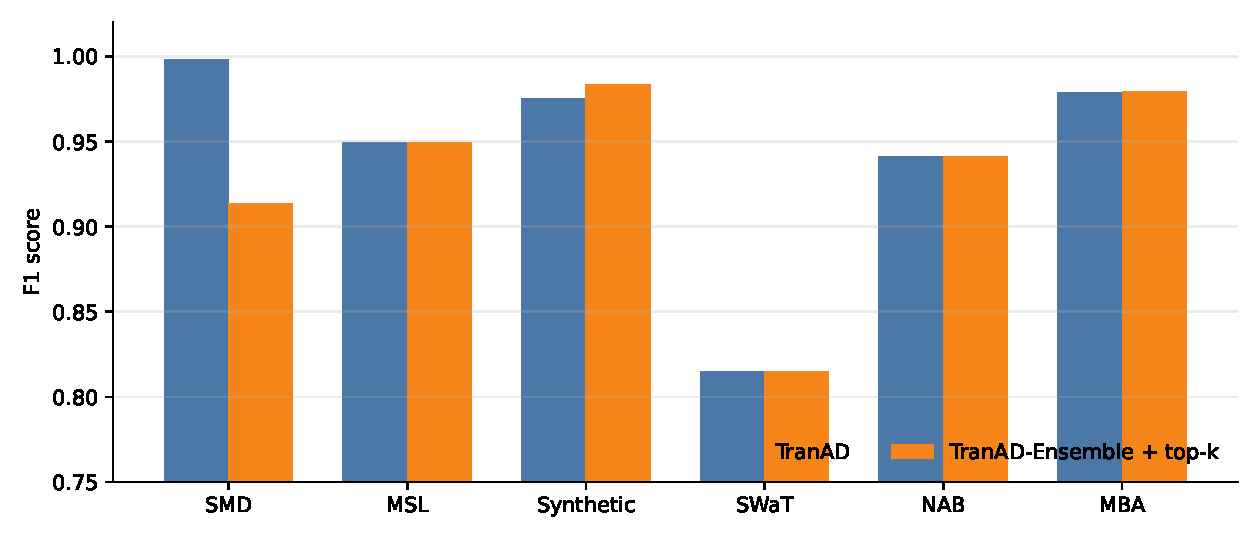
\includegraphics[width=0.92\linewidth]{figures/f1_comparison.pdf}
    \caption{F1 score comparison between TranAD and TranAD-Ensemble with top-k aggregation.}
    \label{fig:f1_comparison}
\end{figure}

\subsection{Metric Differences}

Figure~\ref{fig:metric_delta} shows metric changes relative to TranAD. The primary degradation is the recall drop on SMD. On the remaining datasets, metric changes are either zero or slightly positive.

\begin{figure}[H]
    \centering
    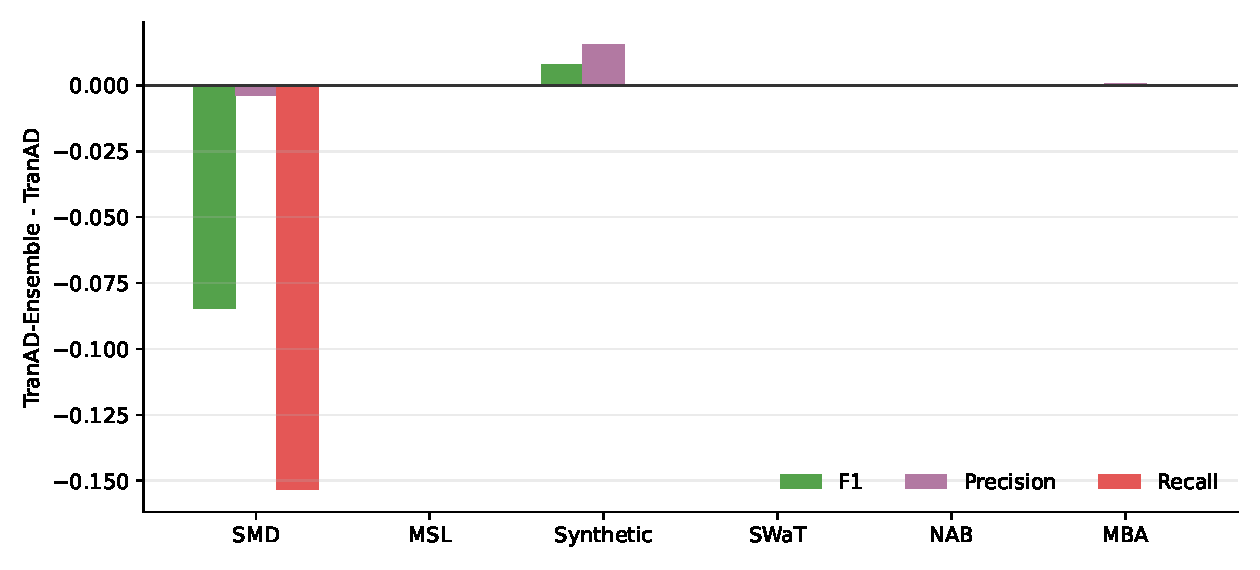
\includegraphics[width=0.92\linewidth]{figures/metric_deltas.pdf}
    \caption{Metric differences of TranAD-Ensemble with top-k aggregation relative to TranAD.}
    \label{fig:metric_delta}
\end{figure}

\section{Discussion}

The results suggest that TranAD-Ensemble with top-k aggregation is not uniformly better than TranAD. Its behavior depends on how anomaly information is distributed across variables.

For Synthetic and MBA, the improvement suggests that localized high-error variables can provide useful anomaly evidence. In these cases, top-k aggregation may reduce the dilution effect caused by averaging over many normal variables.

For MSL, SWaT, and NAB, the final metrics are unchanged. This may indicate that either the detected anomaly regions are already sufficiently strong under the baseline score, or that the top-k aggregation produces nearly equivalent threshold decisions after post-processing.

For SMD, the recall drop is significant. This indicates that top-k aggregation may miss weak or distributed anomalies when abnormal behavior is spread across multiple variables rather than concentrated in a few dominant dimensions. From the perspective of critical transition forecasting, this is an important limitation: some critical transitions may emerge through distributed system-level changes rather than isolated variable spikes.

\section{Stage Conclusion}

This stage completed a focused evaluation of TranAD-Ensemble with top-k aggregation. The main conclusions are:

\begin{enumerate}
    \item TranAD-Ensemble with top-k aggregation provides small improvements on Synthetic and MBA.
    \item It preserves baseline-level performance on MSL, SWaT, and NAB.
    \item It significantly decreases recall on SMD, which is the main current weakness.
    \item The current result supports top-k aggregation as a potentially useful scoring strategy for localized critical-event signals, but not as a universally robust replacement for mean aggregation.
\end{enumerate}

Overall, the current method should be treated as a preliminary stage result. It provides useful evidence for the relationship between localized reconstruction error and critical-event forecasting, but additional robustness analysis is required before claiming general improvement over TranAD.

\section{Next Steps}

Future work should focus on the following tasks:

\begin{itemize}
    \item Perform ablation over different values of $k$ in top-k aggregation.
    \item Compare mean, max, percentile, top-k, and hybrid aggregation strategies.
    \item Analyze SMD false negatives to determine whether degradation is caused by the phase-output ensemble or by top-k aggregation.
    \item Test multiple random seeds and training epochs to separate stable effects from training variance.
    \item Develop an adaptive aggregation mechanism that can switch between localized and distributed anomaly evidence.
    \item Connect anomaly score behavior to critical-event indicators such as persistence, variable coupling, and pre-transition instability.
\end{itemize}

\end{document}
